\documentclass[a4paper, 11pt]{article}
\usepackage{comment} % enables the use of multi-line comments (\ifx \fi) 
\usepackage{lipsum} %This package just generates Lorem Ipsum filler text. 
\usepackage{fullpage} % changes the margin
\usepackage{graphicx}
\usepackage{placeins}
\usepackage{tabto}

\begin{document}
%Header-Make sure you update this information!!!!
\noindent
\begin{center}
      \large\textit{CSE 519}\\
      \Large\textbf{Academic Paper Ranking}\\
\end{center}
\section*{Introduction}
Ranking of academic papers helps scholars to focus on their publishing efforts and can
be widely used for judging the quality of work and research done. There have been numerous approaches to rank these papers, the most traditional being peer grading provided by institutions. But these ranks are divergent to be considered as a standard ranking system. There have been many efforts in the past to make the rankings consistent and relative. The ranking metrics now rely on observed bibliometric measures on the journal-level which is used as representative of quality and eliminates the need of subjective assessment. Taking the example of Google Scholar h-index rankings, it avoids many ‘good’ papers just because of the less number of
citations as it has been experimented many times that their algorithm gives citations the most weightage.We would like address this problem by
devising an algorithm based on several factors like impact factors, Altmetrics, its
scientific and social impact.This report documents the progress that we have done in ranking the academic papers. We explored various data sources and experimented with them. The experiments and why or why not that data set is used is explained in the Data Collection section
. The next section introduces the exploration and the pre-processing done on data. Further sections explains the modeling done on the data and evaluation done. The last section details the next steps for the project.

\section*{Data Collection}
% We have used the ACM version 9 data from Citation Data Network for preliminary data analysis. This data was not complete. It was missing many references and author data. We therefore explored another options to get more data:

% \item DBLP : We have explored the DBLP dataset from Citation Network data to integrate with the ACM, but the integration was a pain consider there were duplicate papers and different format of data for both the datasets.
% \item MAG: Of the various datasets explored, we found the MAG data to be highly rich and organised. This paper supports the analysis: http://www.dlib.org/dlib/september16/herrmannova/09herrmannova.html . We are in the process of getting the full data as it is taking time to download the data via API access.
% \item Altmetrics: We had approached the Altmetrics team to get the altmetric data of the academic papers. We got access to the data on November 13 and we are exploring this data set.
We started with exploring the ACM version 9 data from Citation Data Network. Fig 1 explains the dataset. Almost 50\% of the rows didn't have references. Another 5\% of the data had missing author. The missing reference data was handled by filling the references with the values after max reference of the paper.
\begin{figure}[ht]
\centering
  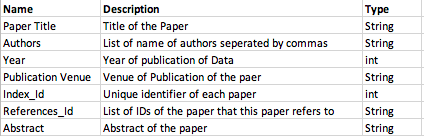
\includegraphics[width=0.7\columnwidth]{ACM_Versio_9_DataSet.png}
  \caption{ACM Version 9}~\label{fig: Microsoft Academic Graph}
\end{figure}
\FloatBarrier
Owning to the missing data in ACM version , we decided to explore the DBLP version 9 data and to merge this data into the ACM dataset. However, the reference id representation in both the data was in an incomparable state and couldn't be merged.
\newline 
To address these issues , we further searched for a better data set and we have come across Microsoft Academic Graph.This dataset is the richest and most comprehensive data till date[1].Fig2 describes the data set that we are downloading from the API . The data was fetched by Microsoft Cognitive Service Labs by using their APIs. The data fetched was in the format of JSON and was converted to CSV.  The limitation here was only 1000 rows can be fetched in a single request to the API. The data was rich in the information as it has categorization of paper, keywords from abstract, proper references, popularity of the paper using Bing's search index. So we went ahead in creating a python script to fetch data from the API. The dataset is rather huge, resulting in million of rows for a single year. To decrease the data download time we used multithreading to concurrently fetch the data.\\
\begin{figure}[ht]
\centering
  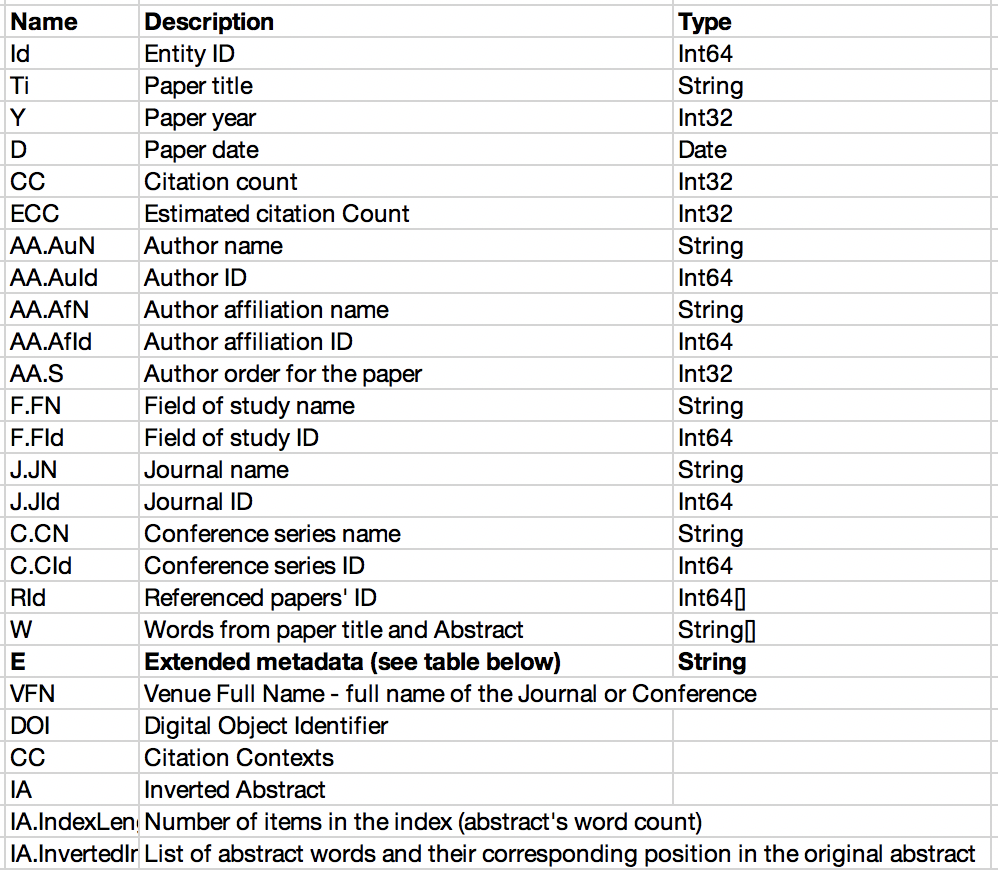
\includegraphics[width=0.7\columnwidth]{MAG_data-info.png}
  \caption{Microsoft Academic Graph}~\label{fig: Microsoft Academic Graph}
\end{figure}
\FloatBarrier

Another set of useful dataset is gathered from Scopus. Scopus contains details of all the major conferences around the world and evaluates rank of publications based on different parameters collected.
\begin{figure}[ht]
\centering
  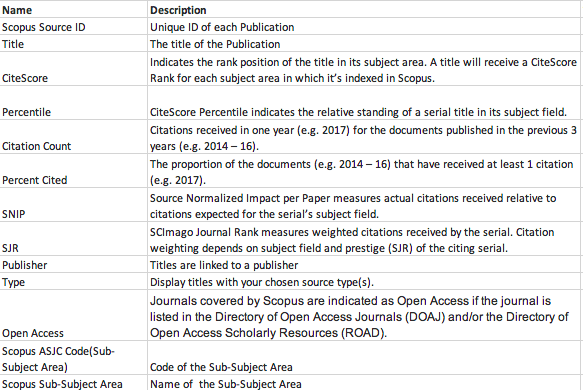
\includegraphics[width=0.7\columnwidth]{Scopus_data_info.png}
  \caption{Microsoft Academic Graph}~\label{fig: Microsoft Academic Graph}
\end{figure}
\FloatBarrier
\section*{Data Exploration on ACM DataSet}
We implemented a function CountReference which counts the number of times a paper is referred. Along with that we calculated outbound references giving us the number of research papers referred by given paper. Then we began analyzing different relations and initial exploratory data analysis. It was observed that number of citation follows Power Law across different research papers. This observation is logical and is in essence the problem with H-index ranking. The papers that are popular gain more traction and keep on getting more citation than other equally good research papers.
\begin{figure}
    \centering
    \begin{minipage}{0.45\textwidth}
        \centering
        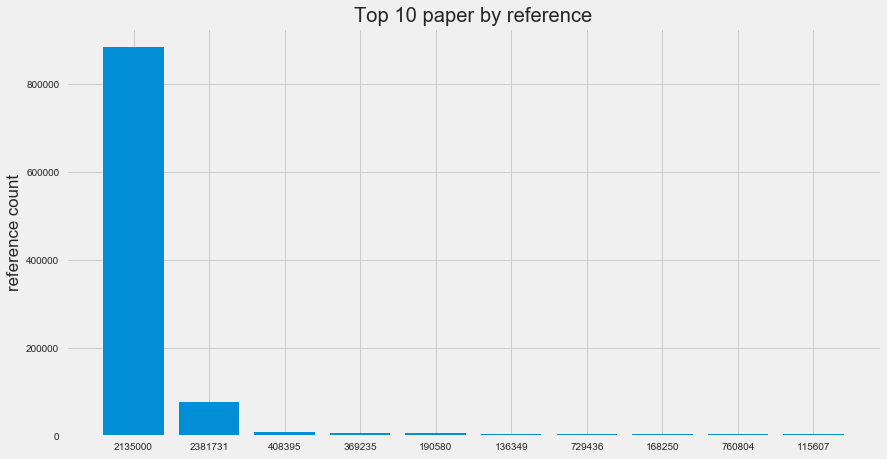
\includegraphics[width=1.1\textwidth]{top_10_papers.png}
        \caption{Number of papers published per year}
    \end{minipage}\hfill
    \begin{minipage}{0.45\textwidth}
        \centering
        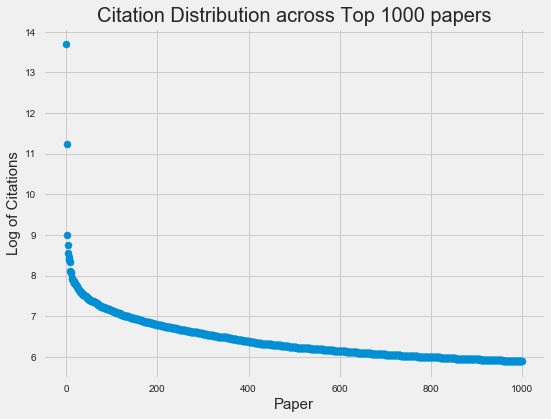
\includegraphics[width=.9\textwidth]{power_law.png}
        \caption{Power Law in action}
    \end{minipage}
\end{figure}
\FloatBarrier
\\

The number of papers published follows a skewed Normal Distribution. The monotonic increment in the number of papers published seems reasonable as the number of domains and research area come up with time. But the decrease in the published paper can only account to improper data collection which neglected the papers published recently in the journal. Another reason behind it can be that the publishing of a paper takes time thus we would be able to see more papers on a later time.

\begin{figure}[ht]
    \centering
    \begin{minipage}{0.45\textwidth}
        \centering
        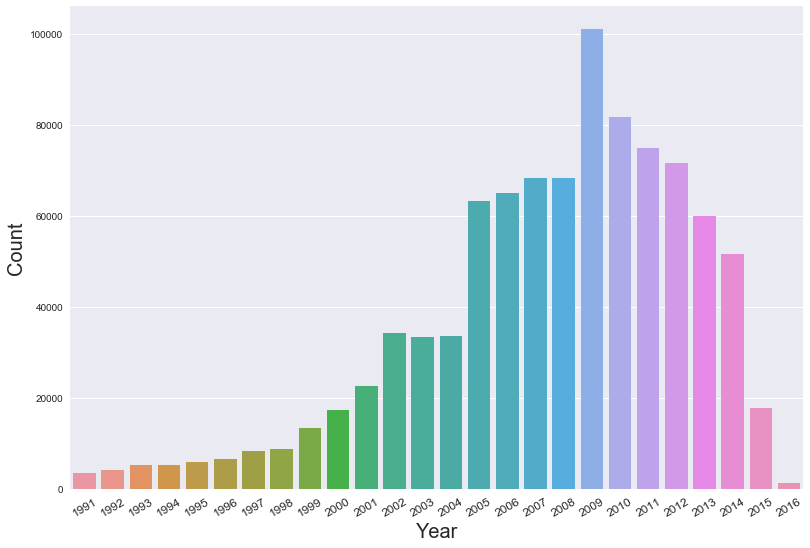
\includegraphics[width=1.2\textwidth]{year-distribution.png}
        \caption{Number of papers published per year}
    \end{minipage}\hfill
    \begin{minipage}{0.45\textwidth}
        \centering
        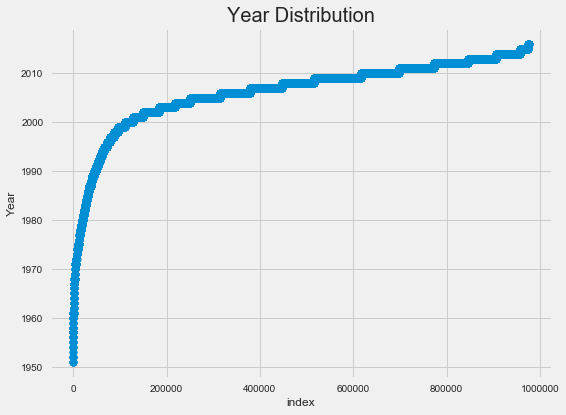
\includegraphics[width=.9\textwidth]{year_graph.png}
        \caption{Paper publication year distribution}
    \end{minipage}
\end{figure}
\FloatBarrier
This is added as a feature and column in the data. We then used PageRank algorithm[2] to rank a paper by considering year, in degree and out degree of the paper.Using the inlinks and outlinks map created, a modified iterative PageRank algorithm is applied to  calculate the authoritative score for each node. In all the iterations, rank of a link is updated using the following formula:
\[ NS = 0.15 + 0.85 * \sum (PR[I]/OC[I]) \]
ie for each link , new score is updated using the number of incoming links and the outgoing links. This score is further normalised using average year citation count. 
% Put page rank graph - TODO
We also calculated number of authors per paper and trained the model with this feature as well. \\
% Put average author graph - TODO
We implemented the reach function which takes a paper as parameter and gives the impact level of the paper. We used DFS to implement the function. 

% PUT GRAPH OF REACH FUNCTION - TODO
\begin{figure}[ht]
  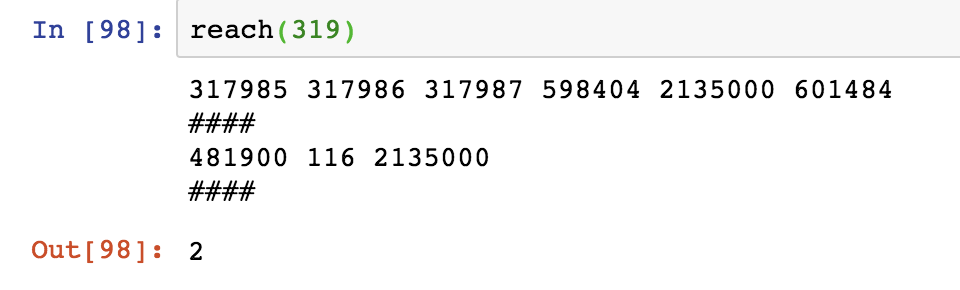
\includegraphics[width=0.6\columnwidth]{Reach.png}
  \caption{Reach of paper indexed 711}~\label{fig:Reach}
\end{figure}
\FloatBarrier
There were some interesting observations.\\

There was one paper with 115 author, this was considered as an outlier since this skewed the average author feature to the right. \\

There were some papers whose reach was as far as \textit{3000} nodes. One of these was  'Basic Concepts in Knowledge Based Systems'
% put the paper name

% \begin{enumerate}
% \item Graph of number of papers vs count of references
% \item Average number of authors of a paper.
% \item One paper with 115 author. interesting?
% \item Co-relation map with page rank?
% \item with geography?
% \end{enumerate}

\section*{Data Exploration and Pre-Processing on MAG DataSet}
Exploring the data distribution: It is interesting to note in the Fig 9 that the number of papers published in January are higher than any other month. This is because a large number of conferences are held in this month.
\begin{figure}[ht]
  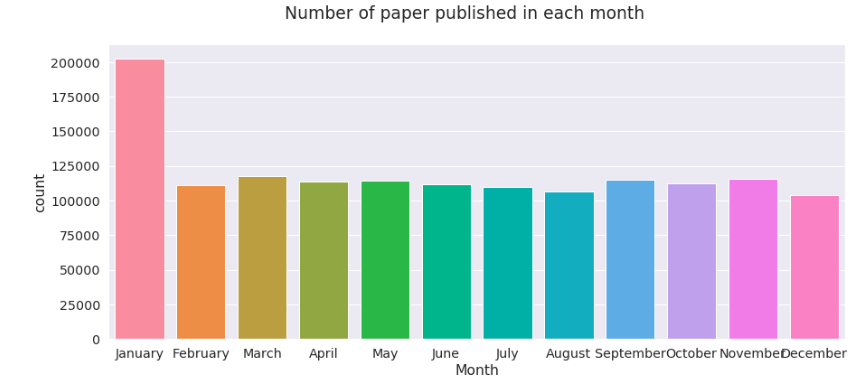
\includegraphics[width=0.6\columnwidth]{Month_Distribution.png}
  \caption{Number of paper published in each month}~\label{fig:Reach}
\end{figure}
\FloatBarrier
\begin{figure}[ht]
  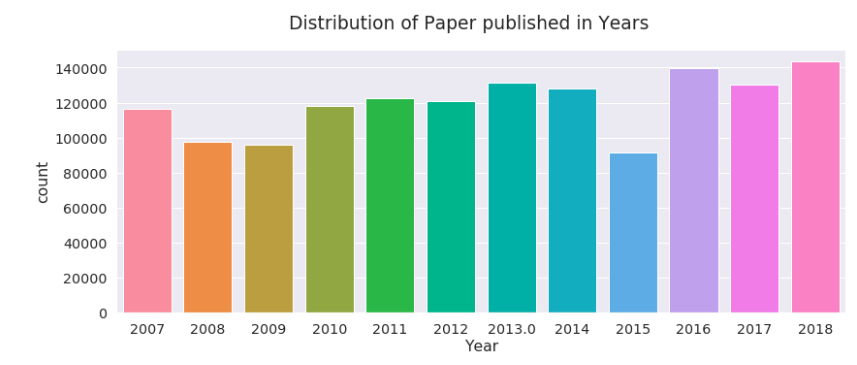
\includegraphics[width=0.6\columnwidth]{Year_Distribution.png}
  \caption{Distribution of papers published in Year}~\label{fig:Reach}
\end{figure}
\FloatBarrier
\begin{figure}[ht]
  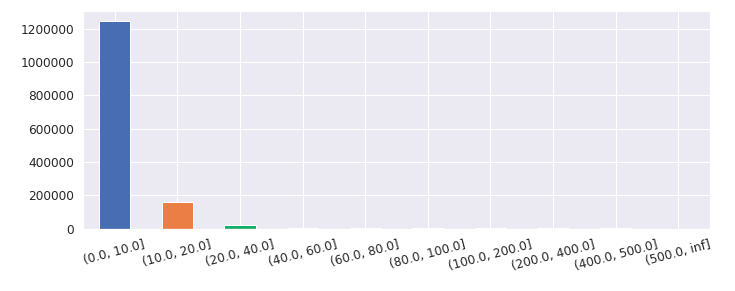
\includegraphics[width=0.6\columnwidth]{Number_Of_Authors.png}
  \caption{Authors per paper}~\label{fig:Reach}
\end{figure}
\FloatBarrier
Since we had a cleaner and better dataset, we didn't have to do much to clean the data. We first merged the Publication data extracted from the Scopus Dataset. For all the publications that were present in the Scopus data, we merged the SJR rank of the publication with our data. The other publications were dropped. We have 1200 such unique publications. We also extracted a lot of features from the existing data.  The features extracted are :\newline
\begin{itemize}
    \item \textbf{Publication Type:} Along with the Publication Venue, we also had information about the Journal and the Conference of the paper. We assigned different Publication types to the feature based on these two columns.
    \begin{table}[h]
  \centering
  \begin{tabular}{l | r | r}
    % \toprule
    {\small \textit{Journal}}& {\small \textit{Conference}} & {\small \textit{Publication Type}}\\
    {\small \textit{Nan}} & {\small \textit{Present}} & {\small \textit{0}}\\
    {\small \textit{Present}} & {\small \textit{Nan}} & {\small \textit{1}}\\
    {\small \textit{Nan}} & {\small \textit{Nan}} & {\small \textit{3}}\\
    {\small \textit{Present}} & {\small \textit{Present}} & {\small \textit{2}}\\
    % \bottomrule
  \end{tabular}
  \caption{Publication Type}~\label{tab:table1}
\end{table}
Most of the papers in our data belong to the Journal type as shown in the following graph.
\begin{figure}[ht]
  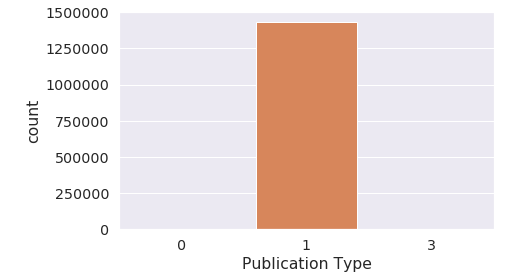
\includegraphics[width=0.6\columnwidth]{PublicationType.png}
  \caption{Publication Type}~\label{fig:Reach}
\end{figure}
\FloatBarrier
    \item \textbf{Number Of Authors}
    \item \textbf{First Author}
    \item \textbf{Page Rank}
    \item \textbf{First Author Rank}
    \item \textbf{Avg Author Rank}
    \item \textbf{Year}
    \item \textbf{Month}
    \item \textbf{Year Since Publication}
    \item \textbf{Domain Count}
\end{itemize}

\section*{Data Modelling}




\section*{Evaluation}


\section*{Next Steps}

% \lipsum[6]



\begin{thebibliography}{9}
\bibitem{Robotics}Drahomira Herrmannova and Petr Knoth \emph{An Analysis of the Microsoft Academic Graph
}
\bibitem{Robotics}Jie Tang, Limin Yao, Duo Zhang, and Jing Zhang. A \emph{ Combination Approach to Web User Profiling. ACM Transactions on Knowledge Discovery from Data (TKDD), (vol. 5 no. 1), Article 2 (December 2010), 44 pages}
\bibitem{Robotics}Arnab Sinha, Zhihong Shen, Yang Song, Hao Ma, Darrin Eide, Bo-June (Paul) Hsu, and Kuansan Wang. 2015. \emph{An Overview of Microsoft Academic Service (MAS) and Applications. In Proceedings of the 24th International Conference on World Wide Web (WWW ’15 Companion). ACM, New York, NY, USA, 243-246}

\bibitem{Robotics}Aditya Pratap Singh 
Centre for Data Engineering, IIIT Hyderabad, India
; Kumar Shubhankar ; Vikram Pudi \emph{An efficient algorithm for ranking research papers based on citation network
}

\end{thebibliography}

\end{document}
